\chapter{The Translating Coil Magnetometer}
The measurement system that will be analyzed in this thesis consists
of a round PCB with multiple different coils. These coils are in the shapes
of disks or annulus segments. A render of the pcb can be seen in figure
\ref{fig:pcb}. The PCB is moved longitudinally inside the magnet aperture,
whereupon the coils pick up the magnetic flux.

\begin{figure}[h]
    \centering
    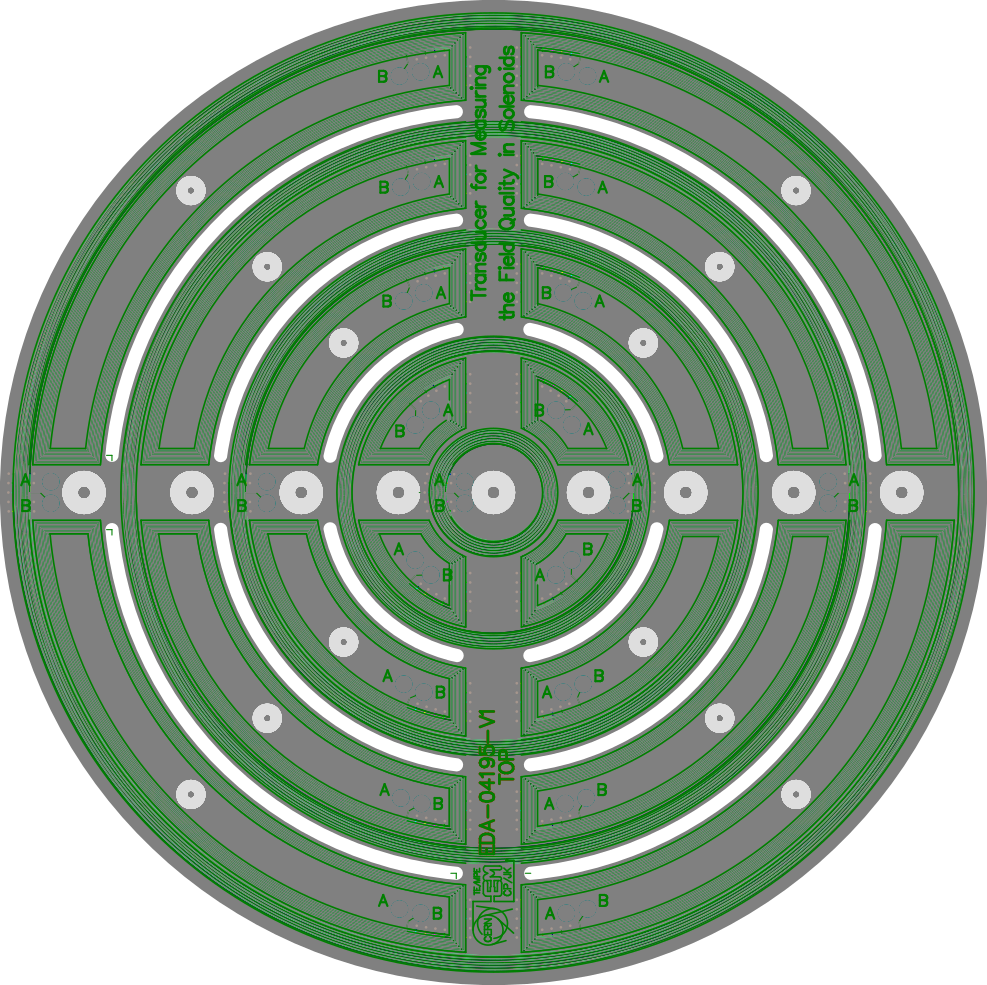
\includegraphics[width=0.5\linewidth]{figs/pcb}
    \caption{The magnetometer PCB.}
    \label{fig:pcb}
\end{figure}

\section{PCB printed coils}
The disks are denoted $D_l$ and the 
annulus segments by $Q_{q, l}$ where $l$ denotes radial layer and 
$q$ denotes quadrant.
\section{Positional Encoder}
\section{Geometric Lidar Measurements}
\section{Fast Digital Integrators}
\section{The Measurement Assembly}